% Options for packages loaded elsewhere
% Options for packages loaded elsewhere
\PassOptionsToPackage{unicode}{hyperref}
\PassOptionsToPackage{hyphens}{url}
\PassOptionsToPackage{dvipsnames,svgnames,x11names}{xcolor}
%
\documentclass[
  letterpaper,
  DIV=11,
  numbers=noendperiod]{scrartcl}
\usepackage{xcolor}
\usepackage[margin=1in]{geometry}
\usepackage{amsmath,amssymb}
\setcounter{secnumdepth}{-\maxdimen} % remove section numbering
\usepackage{iftex}
\ifPDFTeX
  \usepackage[T1]{fontenc}
  \usepackage[utf8]{inputenc}
  \usepackage{textcomp} % provide euro and other symbols
\else % if luatex or xetex
  \usepackage{unicode-math} % this also loads fontspec
  \defaultfontfeatures{Scale=MatchLowercase}
  \defaultfontfeatures[\rmfamily]{Ligatures=TeX,Scale=1}
\fi
\usepackage{lmodern}
\ifPDFTeX\else
  % xetex/luatex font selection
\fi
% Use upquote if available, for straight quotes in verbatim environments
\IfFileExists{upquote.sty}{\usepackage{upquote}}{}
\IfFileExists{microtype.sty}{% use microtype if available
  \usepackage[]{microtype}
  \UseMicrotypeSet[protrusion]{basicmath} % disable protrusion for tt fonts
}{}
\makeatletter
\@ifundefined{KOMAClassName}{% if non-KOMA class
  \IfFileExists{parskip.sty}{%
    \usepackage{parskip}
  }{% else
    \setlength{\parindent}{0pt}
    \setlength{\parskip}{6pt plus 2pt minus 1pt}}
}{% if KOMA class
  \KOMAoptions{parskip=half}}
\makeatother
% Make \paragraph and \subparagraph free-standing
\makeatletter
\ifx\paragraph\undefined\else
  \let\oldparagraph\paragraph
  \renewcommand{\paragraph}{
    \@ifstar
      \xxxParagraphStar
      \xxxParagraphNoStar
  }
  \newcommand{\xxxParagraphStar}[1]{\oldparagraph*{#1}\mbox{}}
  \newcommand{\xxxParagraphNoStar}[1]{\oldparagraph{#1}\mbox{}}
\fi
\ifx\subparagraph\undefined\else
  \let\oldsubparagraph\subparagraph
  \renewcommand{\subparagraph}{
    \@ifstar
      \xxxSubParagraphStar
      \xxxSubParagraphNoStar
  }
  \newcommand{\xxxSubParagraphStar}[1]{\oldsubparagraph*{#1}\mbox{}}
  \newcommand{\xxxSubParagraphNoStar}[1]{\oldsubparagraph{#1}\mbox{}}
\fi
\makeatother


\usepackage{longtable,booktabs,array}
\usepackage{calc} % for calculating minipage widths
% Correct order of tables after \paragraph or \subparagraph
\usepackage{etoolbox}
\makeatletter
\patchcmd\longtable{\par}{\if@noskipsec\mbox{}\fi\par}{}{}
\makeatother
% Allow footnotes in longtable head/foot
\IfFileExists{footnotehyper.sty}{\usepackage{footnotehyper}}{\usepackage{footnote}}
\makesavenoteenv{longtable}
\usepackage{graphicx}
\makeatletter
\newsavebox\pandoc@box
\newcommand*\pandocbounded[1]{% scales image to fit in text height/width
  \sbox\pandoc@box{#1}%
  \Gscale@div\@tempa{\textheight}{\dimexpr\ht\pandoc@box+\dp\pandoc@box\relax}%
  \Gscale@div\@tempb{\linewidth}{\wd\pandoc@box}%
  \ifdim\@tempb\p@<\@tempa\p@\let\@tempa\@tempb\fi% select the smaller of both
  \ifdim\@tempa\p@<\p@\scalebox{\@tempa}{\usebox\pandoc@box}%
  \else\usebox{\pandoc@box}%
  \fi%
}
% Set default figure placement to htbp
\def\fps@figure{htbp}
\makeatother





\setlength{\emergencystretch}{3em} % prevent overfull lines

\providecommand{\tightlist}{%
  \setlength{\itemsep}{0pt}\setlength{\parskip}{0pt}}



 


\KOMAoption{captions}{tableheading}
\makeatletter
\@ifpackageloaded{caption}{}{\usepackage{caption}}
\AtBeginDocument{%
\ifdefined\contentsname
  \renewcommand*\contentsname{Table of contents}
\else
  \newcommand\contentsname{Table of contents}
\fi
\ifdefined\listfigurename
  \renewcommand*\listfigurename{List of Figures}
\else
  \newcommand\listfigurename{List of Figures}
\fi
\ifdefined\listtablename
  \renewcommand*\listtablename{List of Tables}
\else
  \newcommand\listtablename{List of Tables}
\fi
\ifdefined\figurename
  \renewcommand*\figurename{Figure}
\else
  \newcommand\figurename{Figure}
\fi
\ifdefined\tablename
  \renewcommand*\tablename{Table}
\else
  \newcommand\tablename{Table}
\fi
}
\@ifpackageloaded{float}{}{\usepackage{float}}
\floatstyle{ruled}
\@ifundefined{c@chapter}{\newfloat{codelisting}{h}{lop}}{\newfloat{codelisting}{h}{lop}[chapter]}
\floatname{codelisting}{Listing}
\newcommand*\listoflistings{\listof{codelisting}{List of Listings}}
\makeatother
\makeatletter
\makeatother
\makeatletter
\@ifpackageloaded{caption}{}{\usepackage{caption}}
\@ifpackageloaded{subcaption}{}{\usepackage{subcaption}}
\makeatother
\usepackage{bookmark}
\IfFileExists{xurl.sty}{\usepackage{xurl}}{} % add URL line breaks if available
\urlstyle{same}
\hypersetup{
  pdftitle={Where You Actually Feel It},
  colorlinks=true,
  linkcolor={blue},
  filecolor={Maroon},
  citecolor={Blue},
  urlcolor={Blue},
  pdfcreator={LaTeX via pandoc}}


\title{Where You Actually Feel It}
\usepackage{etoolbox}
\makeatletter
\providecommand{\subtitle}[1]{% add subtitle to \maketitle
  \apptocmd{\@title}{\par {\large #1 \par}}{}{}
}
\makeatother
\subtitle{Structural Foundations of Health --- Part 2 of 2}
\author{}
\date{}
\begin{document}
\maketitle


\begin{center}\rule{0.5\linewidth}{0.5pt}\end{center}

\subsection{\texorpdfstring{{\textbf{Last class, in one
slide}}}{Last class, in one slide}}\label{last-class-in-one-slide}

\textbf{Without looking at your notes:} what does it mean that health is
a \emph{staircase} and not a \emph{cliff}?

Turn to your neighbour. Thirty seconds.

Retrieval practice, not review. Take two answers, correct gently, move
on. Target answer: health improves at every step up, so it is not just a
poverty problem.

\begin{center}\rule{0.5\linewidth}{0.5pt}\end{center}

\subsection{\texorpdfstring{{\textbf{Today}}}{Today}}\label{today}

Advantage is distributed unevenly, and the distribution has a history.

\textbf{Today: where you actually feel it.}

\subsubsection{Home}\label{home}

\subsubsection{Work}\label{work}

\subsubsection{Neighbourhood}\label{neighbourhood}

\subsubsection{Policy}\label{policy}

Then: \textbf{how you would study a real community} --- and a group
exercise doing it.

\begin{center}\rule{0.5\linewidth}{0.5pt}\end{center}

\section{\texorpdfstring{{\textbf{1. Home}}}{1. Home}}\label{home-1}

\begin{center}\rule{0.5\linewidth}{0.5pt}\end{center}

\subsection{\texorpdfstring{{\textbf{Housing does three separate
things}}}{Housing does three separate things}}\label{housing-does-three-separate-things}

\begin{itemize}
\tightlist
\item
  \textbf{What it is made of} --- lead, mould, pests, cold
\item
  \textbf{What it costs you} --- rent takes the money that would have
  been food or a co-pay
\item
  \textbf{Whether you get to stay} --- three moves in a year: new
  school, lost doctor, no sleep
\end{itemize}

Only the first is about the building. The other two are \textbf{money}
and \textbf{stability}.

Students default to ``bad housing = mould''. Push them to the second and
third, which do more damage and are less visible.

\begin{center}\rule{0.5\linewidth}{0.5pt}\end{center}

\subsection{\texorpdfstring{{\textbf{One concrete case:
lead}}}{One concrete case: lead}}\label{one-concrete-case-lead}

\begin{center}
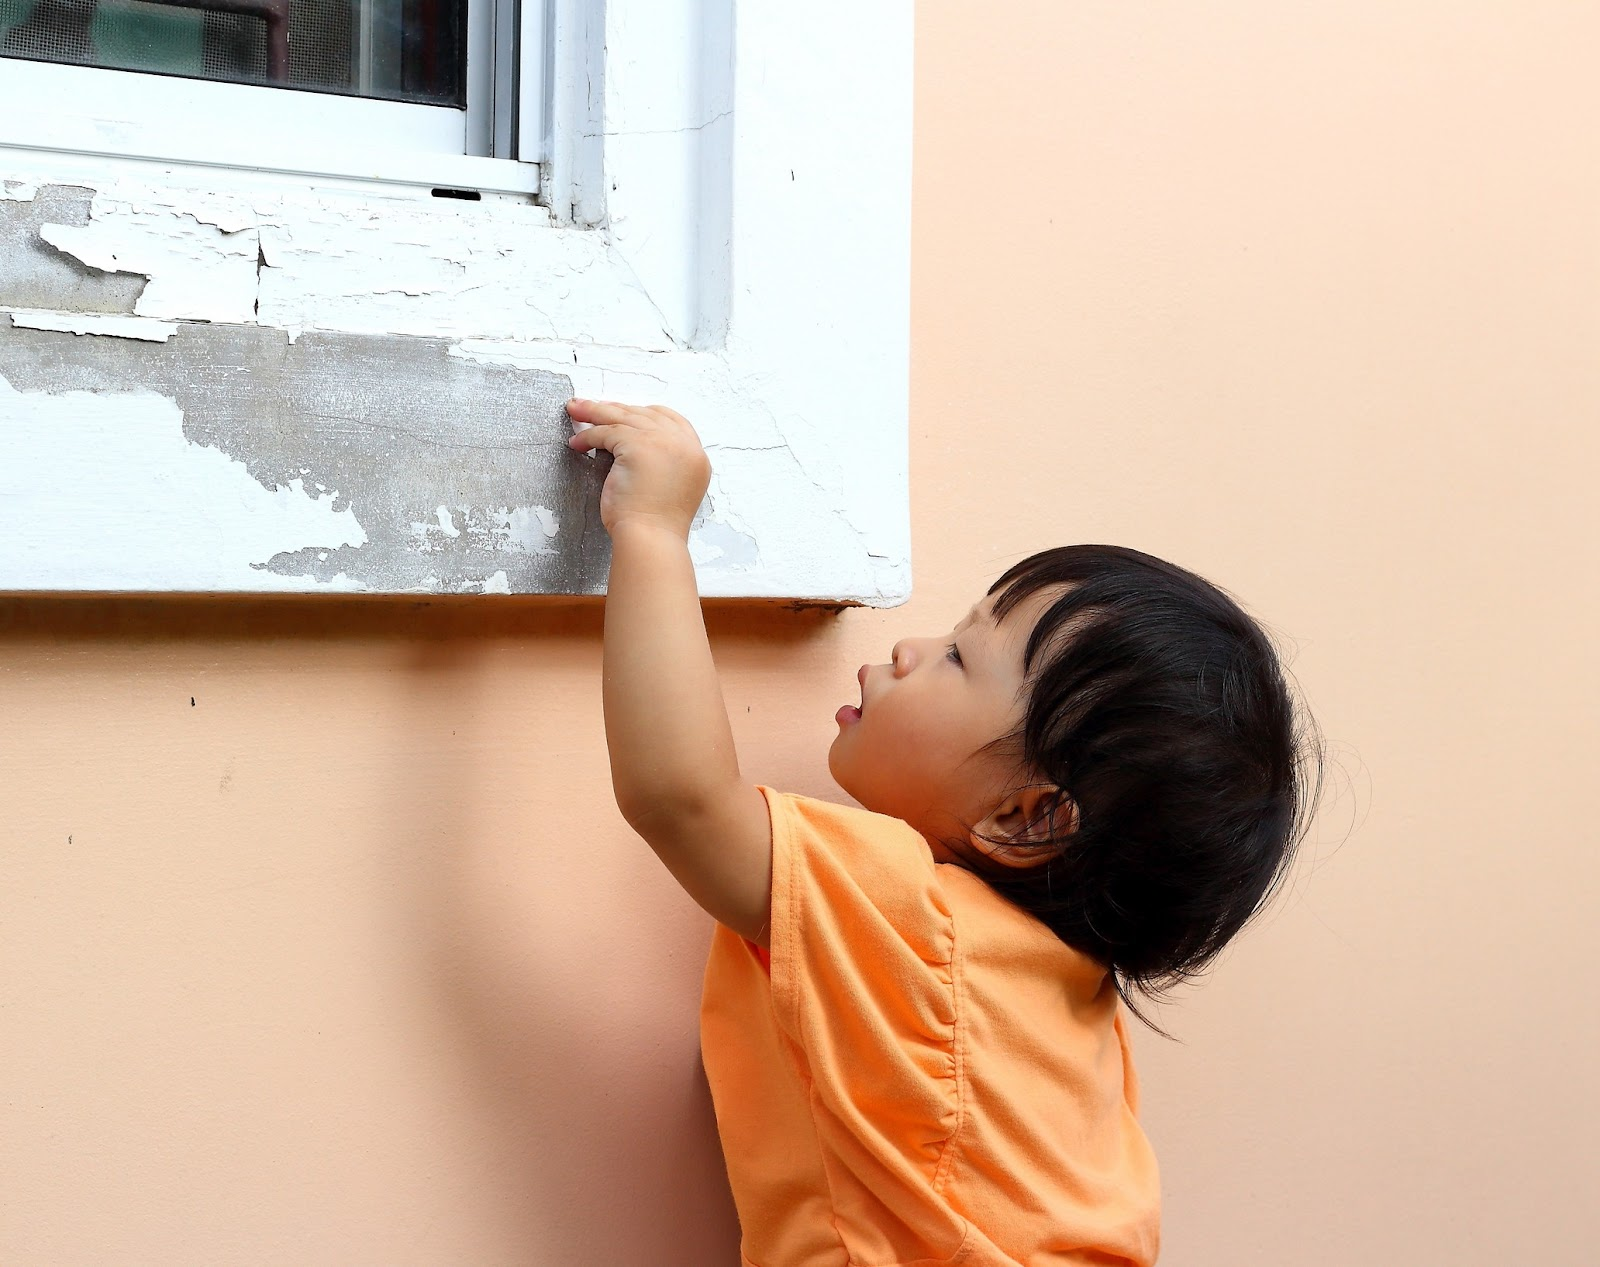
\includegraphics[width=0.48\linewidth,height=\textheight,keepaspectratio]{lead-paint-photo.jpg}
\end{center}

Lead paint was legal in US homes until \textbf{1978} --- and is still in
those walls.

Old housing is concentrated in poor neighbourhoods. Lead damages the
developing brain, and \textbf{the damage does not reverse}.

The cleanest single illustration of the whole course: a 1978 regulation,
a 2026 child, and a mechanism you can draw on the board.

\begin{center}\rule{0.5\linewidth}{0.5pt}\end{center}

\subsection{\texorpdfstring{{\textbf{And the cost
side}}}{And the cost side}}\label{and-the-cost-side}

Paying more than \textbf{30\%} of income on rent =
\textbf{cost-burdened}. Above 50\% = \textbf{severely} cost-burdened.

\textbf{Quick one:} rent goes up \$200 a month, income doesn't. What
comes out of the budget first?

Name three things. Which of them are health?

Expected: groceries, prescriptions, the dentist, the car repair that
gets you to work, heating. All of them are health. This makes housing
cost a health variable, not a finance variable.

\begin{center}\rule{0.5\linewidth}{0.5pt}\end{center}

\section{\texorpdfstring{{\textbf{2. Work}}}{2. Work}}\label{work-1}

\begin{center}\rule{0.5\linewidth}{0.5pt}\end{center}

\subsection{\texorpdfstring{{\textbf{The wrong question and the right
one}}}{The wrong question and the right one}}\label{the-wrong-question-and-the-right-one}

Wrong question: \textbf{do you have a job?}

Right question: \textbf{what does the job do to you?}

Two people both ``employed'' can have completely different health
prospects.

\begin{center}\rule{0.5\linewidth}{0.5pt}\end{center}

\subsection{\texorpdfstring{{\textbf{Three ways a job reaches your
body}}}{Three ways a job reaches your body}}\label{three-ways-a-job-reaches-your-body}

\textbf{The body takes it}

{Lifting, repetition, chemicals, heat}


\includegraphics[width=0.62\linewidth,height=\textheight,keepaspectratio]{heavyboxes.png}

\textbf{The mind takes it}

{High demand, low control, unpredictable hours}

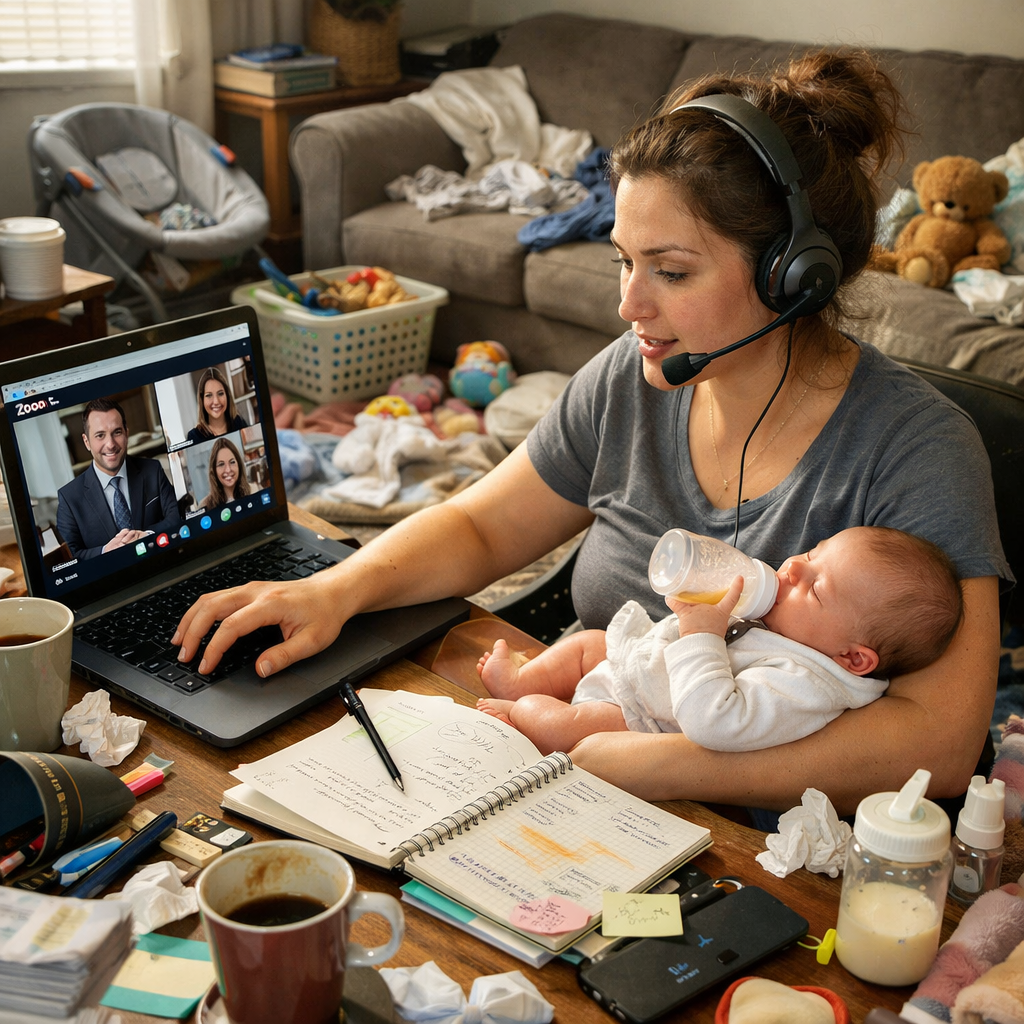
\includegraphics[width=0.62\linewidth,height=\textheight,keepaspectratio]{mother.png}

\textbf{It follows you home}

{Pesticides, solvents, dust on your clothes}

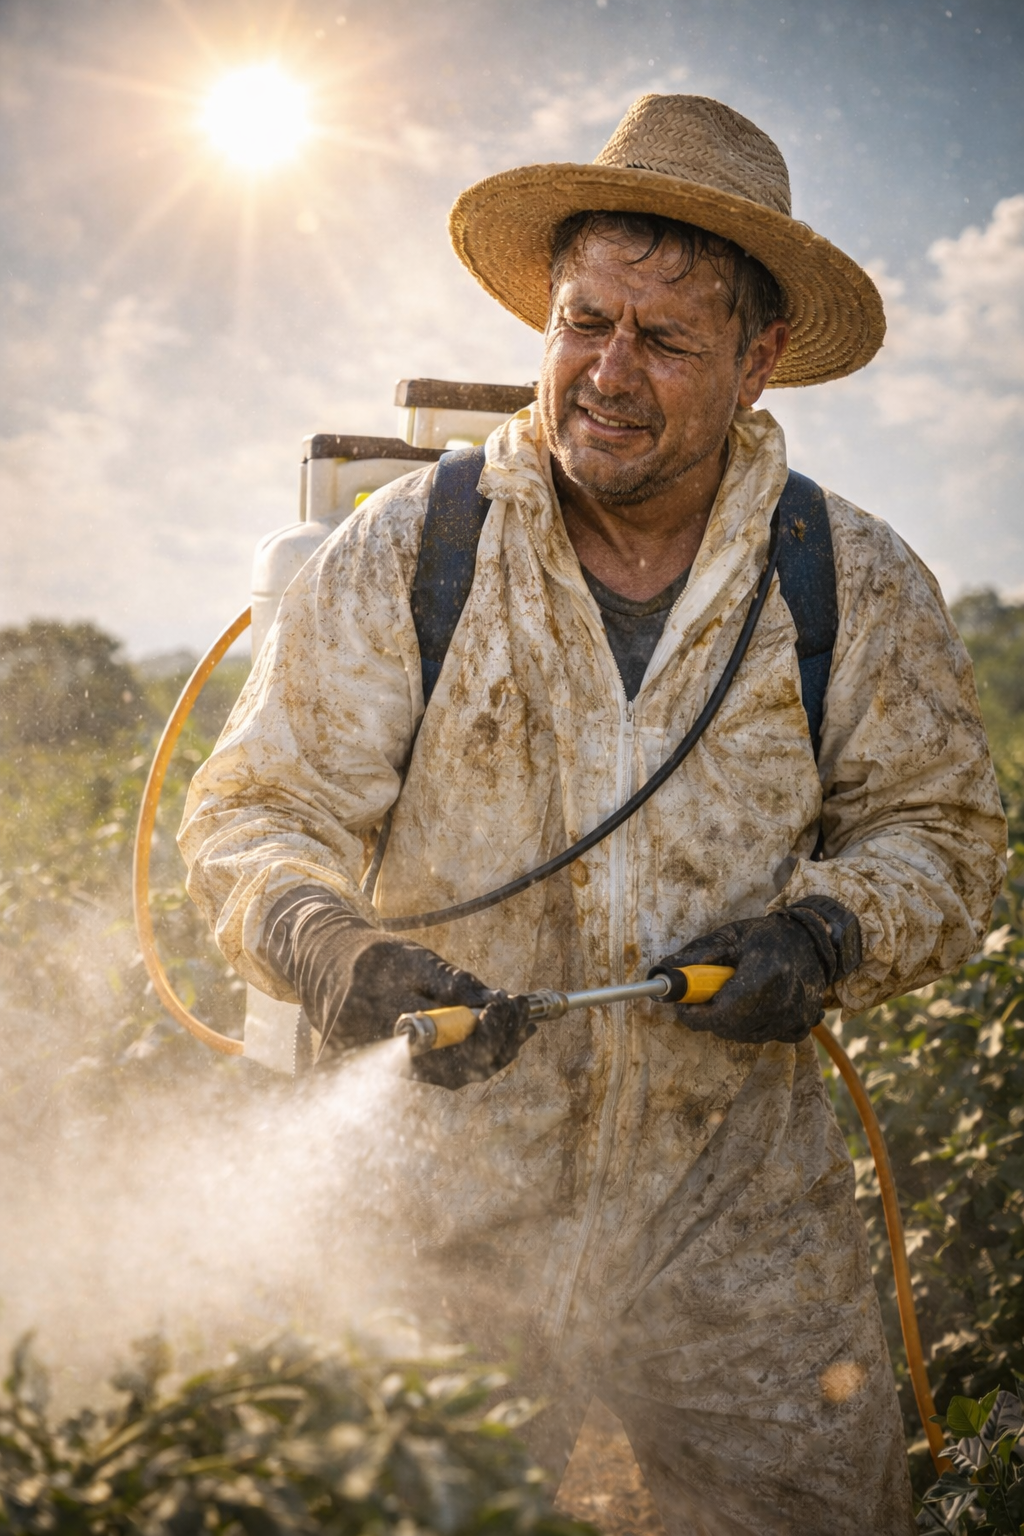
\includegraphics[width=0.62\linewidth,height=\textheight,keepaspectratio]{spray.png}

The middle one is the surprise: \textbf{high demand + low control}
predicts heart disease. Being busy is not the problem. Being busy with
no say is.

\begin{center}\rule{0.5\linewidth}{0.5pt}\end{center}

\subsection{\texorpdfstring{{\textbf{Who actually gets
benefits}}}{Who actually gets benefits}}\label{who-actually-gets-benefits}

\begin{center}
\pandocbounded{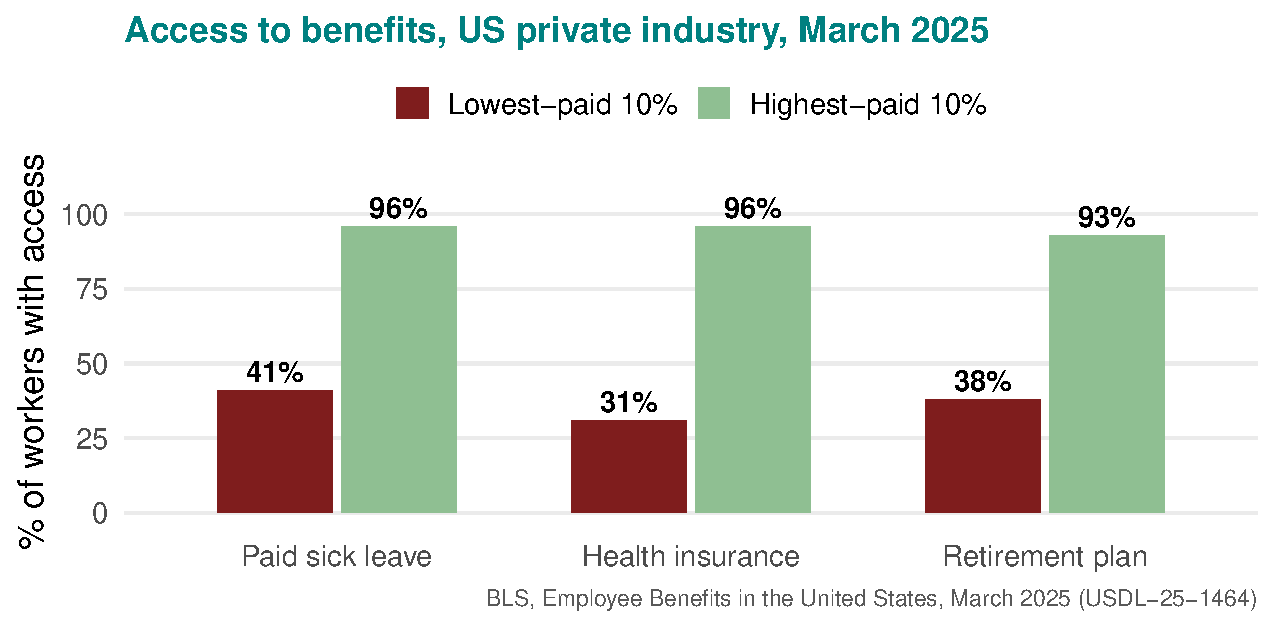
\includegraphics[keepaspectratio]{index_files/figure-pdf/benefits-by-wage-1.pdf}}
\end{center}

``Access'' means the employer offers it, not that the worker takes it up
--- so these bars are the optimistic version.

\begin{center}\rule{0.5\linewidth}{0.5pt}\end{center}

\subsection{\texorpdfstring{{\textbf{Why paid sick leave is a health
policy}}}{Why paid sick leave is a health policy}}\label{why-paid-sick-leave-is-a-health-policy}

\textbf{41\%} of the lowest-paid workers can take a paid sick day.
\textbf{96\%} of the highest-paid can.

So the person handling your food, minding your child, or turning your
grandmother in bed is the one who \textbf{cannot afford to stay home
sick}.

Their working conditions are \textbf{your} exposure. This is why we
study populations, not individuals.

This is the slide that makes the population-level argument land for
students who came in thinking public health is about personal
responsibility.

\begin{center}\rule{0.5\linewidth}{0.5pt}\end{center}

\subsection{\texorpdfstring{{\textbf{And a growing group with none of
it}}}{And a growing group with none of it}}\label{and-a-growing-group-with-none-of-it}

Independent contractors: \textbf{7.4\%} of US employment --- 11.9
million people.

Health insurance from \emph{any} source:

\begin{itemize}
\tightlist
\item
  Traditional employees --- \textbf{85\%}
\item
  Independent contractors --- \textbf{74\%}
\item
  Temp agency workers --- \textbf{61\%}
\end{itemize}

No employer means no employer-sponsored anything: no sick leave, no
workers' comp, no unemployment insurance. \textbf{Insecure work,
insecure health.}

Source: BLS Contingent and Alternative Employment Arrangements, July
2023 (released Nov 2024). Note honestly that BLS does not publish an
employer-coverage figure for contractors, because by definition there is
no employer.

\begin{center}\rule{0.5\linewidth}{0.5pt}\end{center}

\section{\texorpdfstring{{\textbf{3.
Neighbourhood}}}{3. Neighbourhood}}\label{neighbourhood-1}

\begin{center}\rule{0.5\linewidth}{0.5pt}\end{center}

\subsection{\texorpdfstring{{\textbf{What is built around
you}}}{What is built around you}}\label{what-is-built-around-you}

\begin{center}
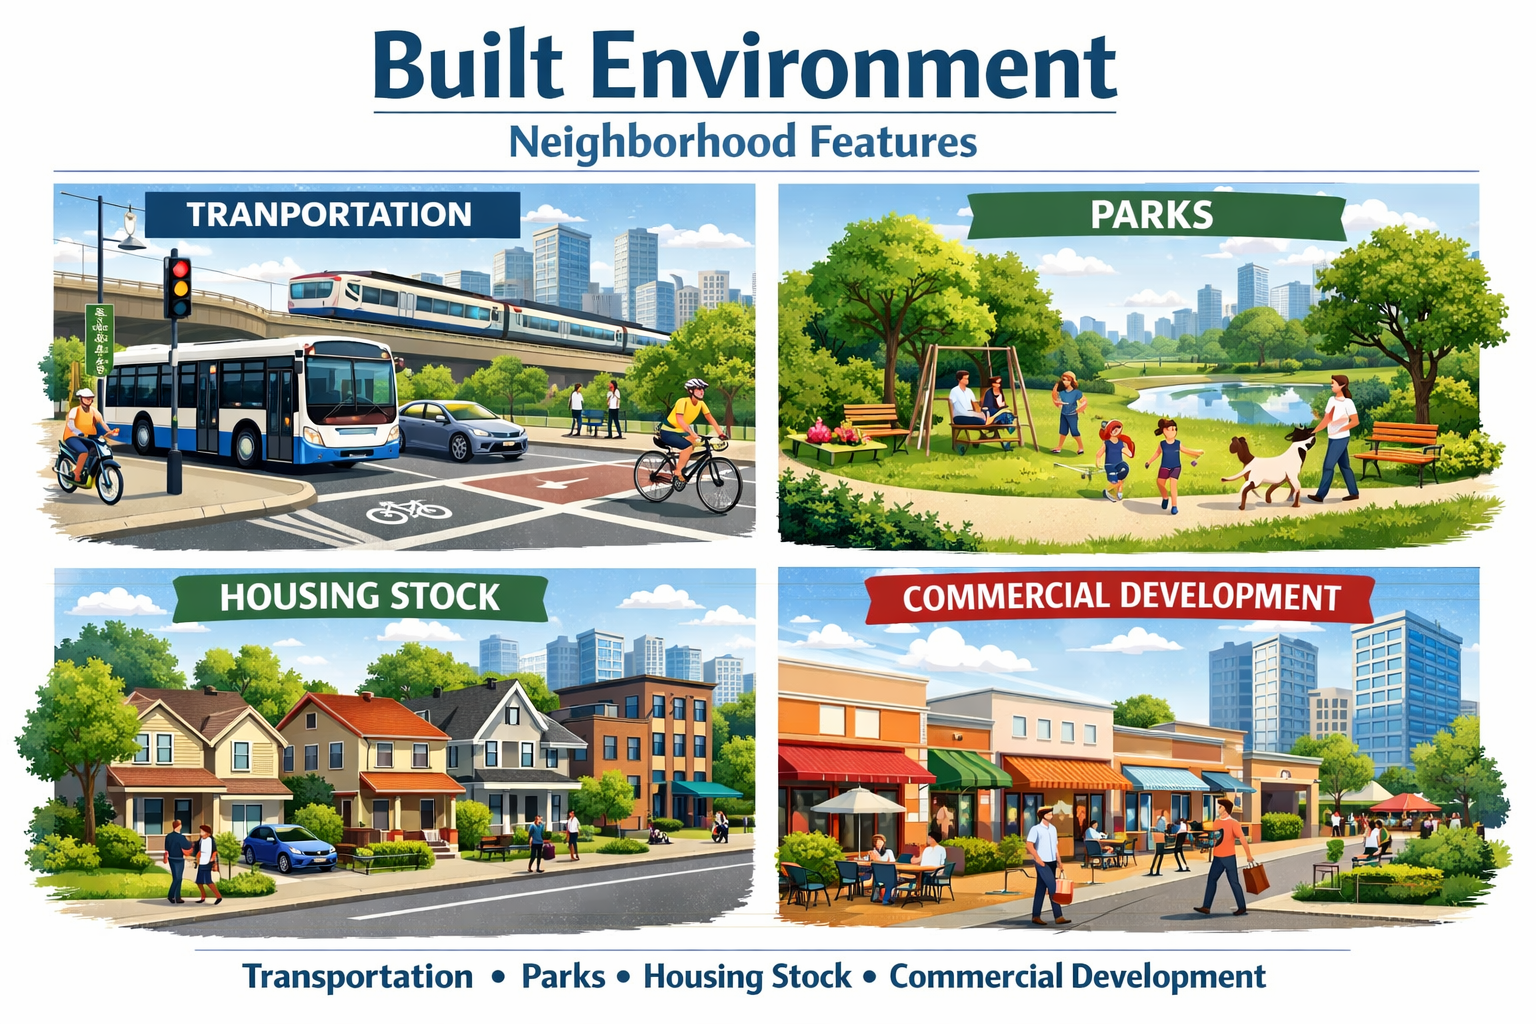
\includegraphics[width=0.68\linewidth,height=\textheight,keepaspectratio]{built-environment.png}
\end{center}

Ask what they can see: sidewalks, crossings, lighting, shade, benches,
whether the shop is walkable. The point is that ``exercise'' is a design
outcome, not only a willpower outcome.

\begin{center}\rule{0.5\linewidth}{0.5pt}\end{center}

\subsection{\texorpdfstring{{\textbf{And what is put near
you}}}{And what is put near you}}\label{and-what-is-put-near-you}

{\textbf{Environmental justice}}: pollution, heat and industrial hazards
are not spread evenly --- they concentrate in low-income neighbourhoods
and neighbourhoods of colour.

Remember last class: \textbf{cheap land is where the highway goes.}

\textbf{Which came first} --- the polluting plant, or the poor
neighbourhood around it?

There is evidence for both. Why does the answer matter for policy?

Genuinely contested in the literature (siting vs.~subsequent demographic
change). Use it to show that ``which came first'' changes whether the
remedy is siting rules or cleanup and relocation.

\begin{center}\rule{0.5\linewidth}{0.5pt}\end{center}

\subsection{\texorpdfstring{{\textbf{What it
does}}}{What it does}}\label{what-it-does}

\begin{itemize}
\tightlist
\item
  \textbf{Lungs} --- asthma, COPD; children worst affected
\item
  \textbf{Heart} --- fine particulate exposure raises cardiovascular
  risk
\item
  \textbf{Heat} --- less shade, more asphalt; heatwave deaths cluster in
  the same blocks
\item
  \textbf{Mind} --- noise, no green space, and knowing this was allowed
  to happen here
\end{itemize}

This is the redlining map again, wearing a different coat.

\begin{center}\rule{0.5\linewidth}{0.5pt}\end{center}

\section{\texorpdfstring{{\textbf{4.
Policy}}}{4. Policy}}\label{policy-1}

\begin{center}\rule{0.5\linewidth}{0.5pt}\end{center}

\subsection{\texorpdfstring{{\textbf{The
lever}}}{The lever}}\label{the-lever}

Home, work and neighbourhood are all \textbf{downstream of decisions
somebody made}.

\textbf{Pushes health up}

\begin{itemize}
\tightlist
\item
  Income support (EITC)
\item
  Medicaid expansion
\item
  Paid leave laws
\item
  Lead abatement funding
\end{itemize}

\textbf{Pushes health down}

\begin{itemize}
\tightlist
\item
  Zoning that blocks affordable housing
\item
  Mass incarceration
\item
  Weak housing-code enforcement
\end{itemize}

None of these is called a health policy. All of them are.

\begin{center}\rule{0.5\linewidth}{0.5pt}\end{center}

\subsection{\texorpdfstring{{\textbf{A natural experiment: Medicaid
expansion}}}{A natural experiment: Medicaid expansion}}\label{a-natural-experiment-medicaid-expansion}

In 2014, some states expanded Medicaid and some did not. Same country,
same decade.

9.4\%

Reduction in annual mortality among low-income adults aged 55--64 in
expansion states.

Miller, Johnson \& Wherry (2021), Quarterly Journal of Economics. Be
precise about the population: low-income adults aged 55--64, not
everybody. Rising to 11.9\% by the third year. Roughly 15,600 deaths
would have been averted had all states expanded.

\begin{center}\rule{0.5\linewidth}{0.5pt}\end{center}

\subsection{\texorpdfstring{{\textbf{And the rest of the
picture}}}{And the rest of the picture}}\label{and-the-rest-of-the-picture}

\begin{center}
\pandocbounded{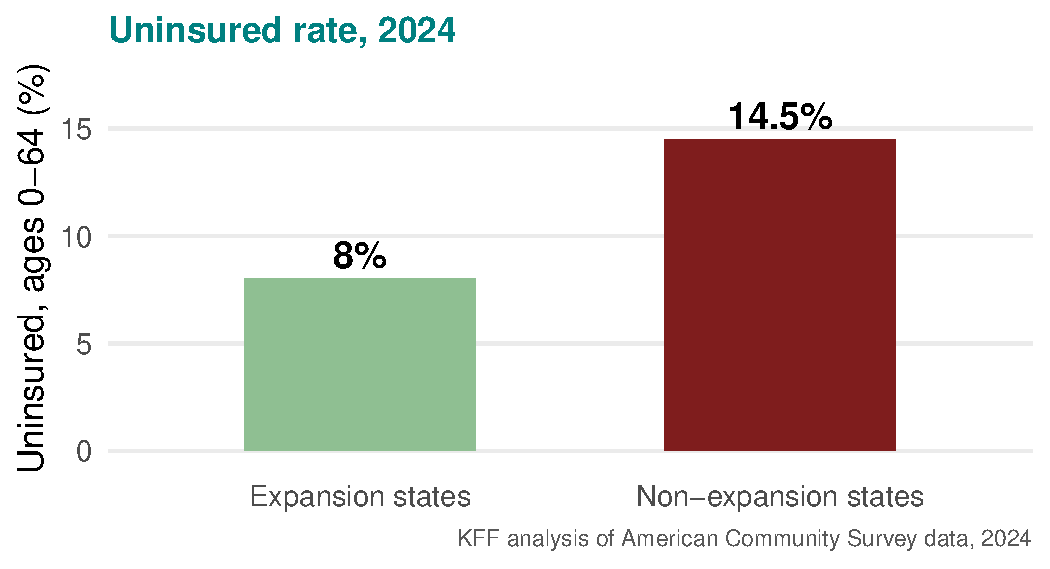
\includegraphics[keepaspectratio]{index_files/figure-pdf/uninsured-by-expansion-1.pdf}}
\end{center}

Expansion also cut medical debt sent to collections by about
\textbf{42\%} (Hu et al.~2018).

Flag the honest caveat: the uninsured bars are a cross-section, not a
causal estimate --- expansion and non-expansion states differ in many
ways. The mortality and debt figures are the causal ones.

\begin{center}\rule{0.5\linewidth}{0.5pt}\end{center}

\section{\texorpdfstring{{\textbf{How would you study a
community?}}}{How would you study a community?}}\label{how-would-you-study-a-community}

\begin{center}\rule{0.5\linewidth}{0.5pt}\end{center}

\subsection{\texorpdfstring{{\textbf{Two different
jobs}}}{Two different jobs}}\label{two-different-jobs}

\subsubsection{Community assessment}\label{community-assessment}

\textbf{One place, in depth.}

\begin{itemize}
\tightlist
\item
  You go there; you talk to people
\item
  Assets as well as problems
\item
  Ends with: a plan somebody can act on
\end{itemize}

\subsubsection{Population assessment}\label{population-assessment}

\textbf{Many places, from above.}

\begin{itemize}
\tightlist
\item
  Registries, surveys, vital statistics
\item
  Compare counties, states, countries
\item
  Ends with: a pattern, and where to look next
\end{itemize}

Neither is better. Each is bad at the other's question.

\begin{center}\rule{0.5\linewidth}{0.5pt}\end{center}

\subsection{\texorpdfstring{{\textbf{Same city, two
questions}}}{Same city, two questions}}\label{same-city-two-questions}

\begin{itemize}
\item
  \textbf{Population:} \emph{Which PA counties have the highest diabetes
  rates?} → surveillance data, a map, a ranking
\item
  \textbf{Community:} \emph{Why this neighbourhood, and what already
  exists here that could help?} → walk the streets, count the shops, ask
  the clinic
\end{itemize}

\textbf{Your individual paper is a community assessment} --- of your own
hometown. That is why it cannot be written from data alone.

Deliberate hook to the individual paper due 24 November. Point out that
the observation part is what earns the marks.

\begin{center}\rule{0.5\linewidth}{0.5pt}\end{center}

\section{\texorpdfstring{{\textbf{Group
exercise}}}{Group exercise}}\label{group-exercise}

\begin{center}\rule{0.5\linewidth}{0.5pt}\end{center}

\subsection{\texorpdfstring{{\textbf{Your
community}}}{Your community}}\label{your-community}

Each group gets one:

\begin{itemize}
\tightlist
\item
  A \textbf{rural coal town} after the mine closed
\item
  An \textbf{urban neighbourhood} with no supermarket
\item
  A recent \textbf{immigrant community}
\end{itemize}

\begin{itemize}
\tightlist
\item
  A \textbf{tribal reservation}
\item
  A \textbf{gentrifying neighbourhood}
\end{itemize}

Hand out the one-page scenarios. Five groups; combine if the class is
small.

\begin{center}\rule{0.5\linewidth}{0.5pt}\end{center}

\subsection{\texorpdfstring{{\textbf{What to do --- 15
minutes}}}{What to do --- 15 minutes}}\label{what-to-do-15-minutes}

\begin{enumerate}
\def\labelenumi{\arabic{enumi}.}
\item
  \textbf{Find three things} making people in your community sicker. One
  must be \emph{home}, \emph{work} or \emph{neighbourhood}.
\item
  \textbf{Trace one backwards.} What decision, by whom, put it there?
\item
  \textbf{Propose one change.} Say who has the power to make it.
\end{enumerate}

Be specific. ``Improve access to healthy food'' is not an answer. ``Move
the bus stop'' might be.

\begin{center}\rule{0.5\linewidth}{0.5pt}\end{center}

\subsection{\texorpdfstring{{\textbf{Then report back --- 2 minutes
each}}}{Then report back --- 2 minutes each}}\label{then-report-back-2-minutes-each}

Tell us:

\begin{itemize}
\tightlist
\item
  Your community, in one sentence
\item
  Your \textbf{three} problems
\item
  The \textbf{one} change you would make, and \textbf{who} would have to
  make it
\end{itemize}

Everyone else: listen for a problem that appears in \textbf{more than
one} community. Those are the structural ones.

The cross-scenario pattern is the payoff. Housing cost, transport and
job insecurity should appear in nearly all five --- which is the
argument of both lectures, arrived at by the students rather than by me.

\begin{center}\rule{0.5\linewidth}{0.5pt}\end{center}

\subsection{\texorpdfstring{{\textbf{Where this goes
next}}}{Where this goes next}}\label{where-this-goes-next}

\begin{itemize}
\tightlist
\item
  \textbf{Tuesday 8 Sept:} Quiz 1, then \textbf{theories and frameworks}
\item
  Groups formed, topics assigned, peer pairings announced
\item
  \textbf{Read:} Chapter 4, sections on determinants
\item
  \textbf{Assignment 1 due Friday 11 September}, midnight
\end{itemize}

\begin{center}\rule{0.5\linewidth}{0.5pt}\end{center}

\section{\texorpdfstring{{\textbf{Now: into your
groups}}}{Now: into your groups}}\label{now-into-your-groups}




\end{document}
